\section{Related work}
\label{ea:sec:related}


Clustering enables to preserve energy for the sensing nodes and offers an easier management of the nodes.
In our case, all nodes of a cluster can reach their \ch directly (\emph{1-hop transmission}), as on \figurename~\ref{ea:fig:wsn}.
\begin{figure}[h]
    \centering
    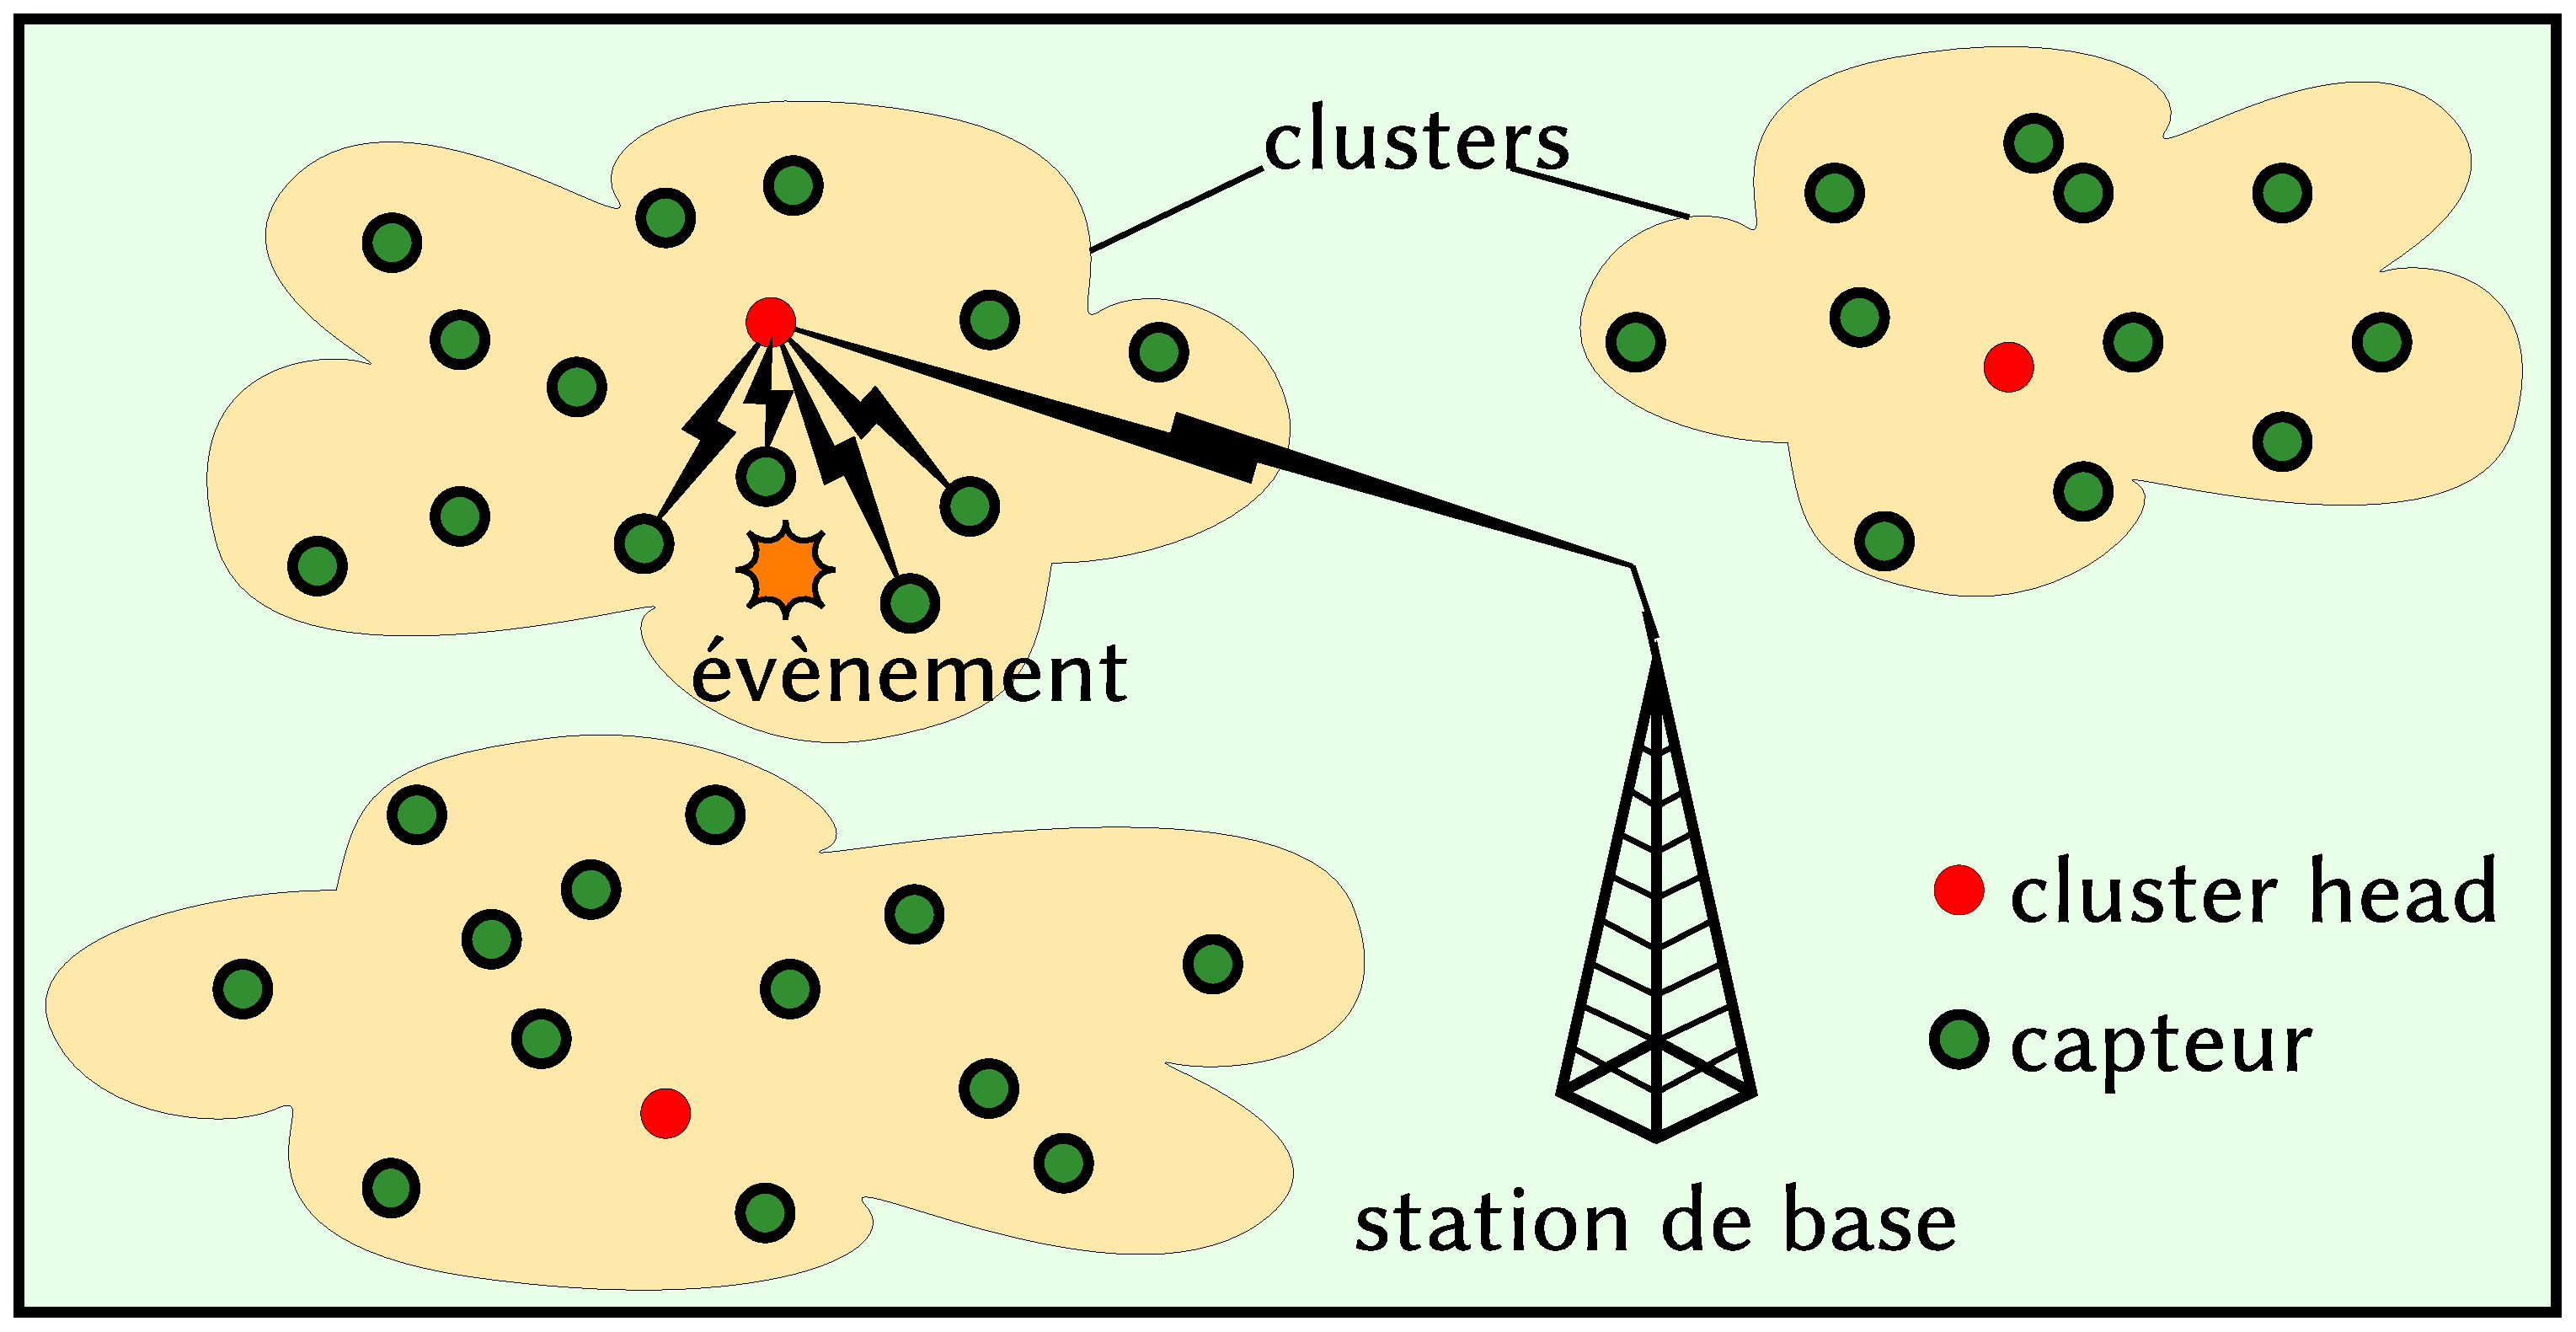
\includegraphics[width=0.8\linewidth]{\chapterfig/WSN.eps}
    \caption{Clustered wireless sensor networks scheme}\label{ea:fig:wsn}
\end{figure}

Control nodes are elected among the non-\ch nodes of a cluster.
We will call them \cns from now on.
They are responsible for listening to the traffic and detecting nodes whose emitted traffic exceeds a given threshold value.
These abnormal behaviors are reported to the \ch.
On reception of reports from several distinct \cns (to prevent false denunciation from a compromised node), the \CH virtually excludes the suspicious node from the cluster.
Although the method is efficient for detecting rogue nodes, the authors do not give details of the election mechanism to choose the \cns.
Also, there is no mention in their study of renewing the election in time, which causes the appointed \cns to endorse a heavier energy consumption on a long period.

